\begin{comment}
\subsection{UC30 - Visualizzazione ristoranti (per amministratore)}\label{usecase:30}

\begin{figure}[H]
    \centering
    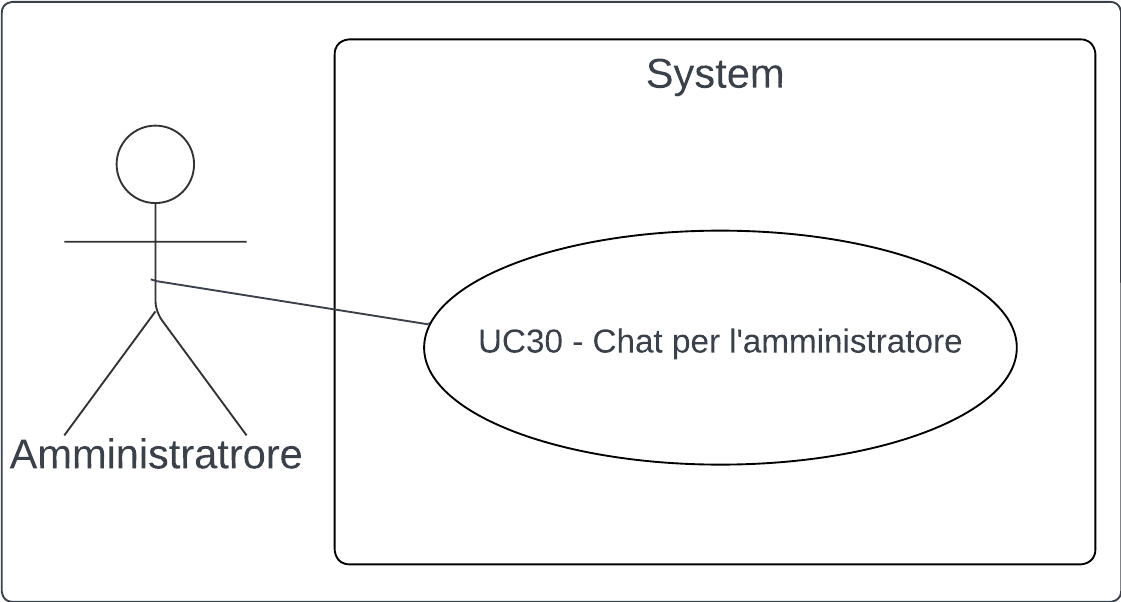
\includegraphics[width=0.9\linewidth]{ucd/UCD30.png}
\end{figure}

\textbf{Attori}:
\begin{itemize}
    \item Amministratore
\end{itemize}
\textbf{Precondizioni}:
\begin{itemize}
    \item L'amministratore è autenticato nel sistema
\end{itemize}
\textbf{Postcondizioni}:
\begin{itemize}
    \item L'amministratore ha visualizzato l'elenco dei ristoranti
\end{itemize}
\textbf{Scenario principale}:
\begin{enumerate}
    \item L'amministratore seleziona l'opzione per visualizzare l'elenco dei ristoranti di cui è l'amministratore
    \item Il $\textit{Sistema}_G$ visualizza l'elenco dei ristoranti
\end{enumerate}
\textbf{Scenari alternativi}:\\
\textit{Nessun ristorante registrato}:
\begin{enumerate}
    \item Dopo il recupero dell'elenco dei ristoranti, il $\textit{Sistema}_G$ non trova alcun ristorante registrato
    \item Il $\textit{Sistema}_G$ visualizza un messaggio all'amministratore indicando che non ci sono ristoranti registrati nel $\textit{Sistema}_G$
\end{enumerate}

\newpage
\end{comment}
\subsection{UC30 - Chat per l'amministratore}\label{usecase:30}
\begin{figure}[H]
    \centering
    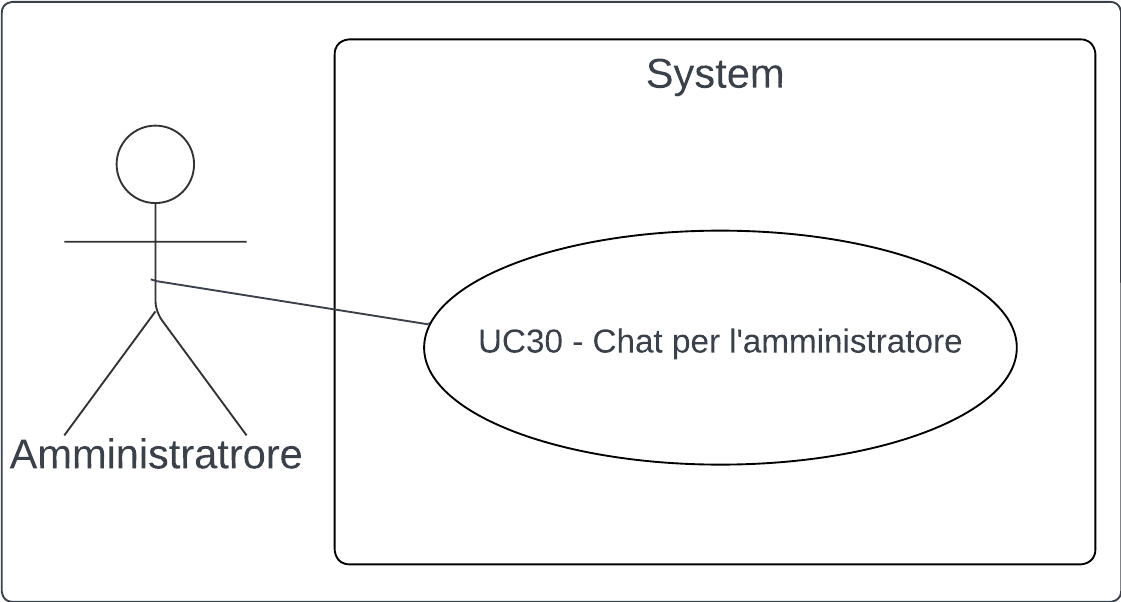
\includegraphics[width=0.75\linewidth]{ucd/UCD30.png}
\end{figure}
\textbf{Attori}:
\begin{itemize}
    \item Amministratore
\end{itemize}
\textbf{Precondizioni}:
\begin{itemize}
    \item L'amministratore amministra un ristorante
\end{itemize}
\textbf{Postcondizioni}:
\begin{itemize}
    \item L'amministratore visualizza una chat per rispondere ad eventuali utenti che hanno scritto
\end{itemize}
\textbf{Scenario principale}:
\begin{enumerate}
    \item L'amministratore visualizza una lista di chat che gli utenti hanno aperto
    \item Seleziona una chat
    \item Visualizza il testo
    \item L'amministratore può rispondere tramite testo
\end{enumerate}
\textbf{Scenari alternativi}:
\begin{enumerate}
    \item Il testo inserito è:
    \begin{enumerate}
        \item Vuoto
        \item Troppo lungo
    \end{enumerate}
    \item L'invio viene annullato e viene visualizzato un errore
\end{enumerate}